\documentclass[9pt,aspectratio=169,xcolor=table]{beamer}

%~~~~~~~~~~~~~~~~~~~~~~~~~~~~~~~~~~~~~~~~~~~~~~~~~~~~~~~~~~~~~~~~~~~~~~~~~~~~~~
% Use roboto Font (recommended)
\usepackage[sfdefault]{roboto}
\usepackage[utf8]{inputenc}
\usepackage[T1]{fontenc}
%~~~~~~~~~~~~~~~~~~~~~~~~~~~~~~~~~~~~~~~~~~~~~~~~~~~~~~~~~~~~~~~~~~~~~~~~~~~~~~

%~~~~~~~~~~~~~~~~~~~~~~~~~~~~~~~~~~~~~~~~~~~~~~~~~~~~~~~~~~~~~~~~~~~~~~~~~~~~~~
% Define where theme files are located. ('/styles')
\usepackage{styles/fluxmacros}
\usefolder{styles}
% Use Flux theme v0.1 beta
% Available style: asphalt, blue, red, green, gray
\usetheme[style=hunter]{flux}
%~~~~~~~~~~~~~~~~~~~~~~~~~~~~~~~~~~~~~~~~~~~~~~~~~~~~~~~~~~~~~~~~~~~~~~~~~~~~~~

%~~~~~~~~~~~~~~~~~~~~~~~~~~~~~~~~~~~~~~~~~~~~~~~~~~~~~~~~~~~~~~~~~~~~~~~~~~~~~~
% Extra packages
\usepackage{booktabs}
\usepackage{colortbl}
\usepackage{ragged2e}
\usepackage{amssymb}
\usepackage{multirow}
\usepackage{tikz}
\usetikzlibrary{arrows.meta, positioning, fit, backgrounds, calc, decorations.pathreplacing}
\setbeamertemplate{itemize items}[square]
\usepackage[scaled=.8]{beramono}
\usepackage{listings}
\usepackage{styles/lstlangarm}
\usepackage{array}
\definecolor{bgcolor}{HTML}{F2E9E9}
% lstlangarm.sty references \color{mauve} for string literals but never defines
% it -- only fires when a listing contains a string. Define it here.
\definecolor{mauve}{rgb}{0.58,0,0.82}
% lstlangarm's C style sets commentstyle=green!20, which is unreadable on the
% pink listing background. Darken it globally.
\lstset{commentstyle=\color{green!45!black}}
% ragged-right fixed-width column -- must be defined in the preamble, never
% inside a frame (\newcolumntype's #1 breaks beamer's frame scanner)
\newcolumntype{R}[1]{>{\RaggedRight\arraybackslash}p{#1}}
%~~~~~~~~~~~~~~~~~~~~~~~~~~~~~~~~~~~~~~~~~~~~~~~~~~~~~~~~~~~~~~~~~~~~~~~~~~~~~~
% Table striping: odd rows white, even rows very light gray.
% Needs \documentclass[...,xcolor=table]{beamer} (beamer loads xcolor itself,
% so the option must go on the class, not \usepackage).
\definecolor{stripe}{gray}{0.94}
% \striped makes body rows alternate white, gray, white, ... starting white.
% \rowcolors counts from the first coloured body row; the header is not counted.
\newcommand{\striped}{\rowcolors{1}{white}{stripe}}
%~~~~~~~~~~~~~~~~~~~~~~~~~~~~~~~~~~~~~~~~~~~~~~~~~~~~~~~~~~~~~~~~~~~~~~~~~~~~~~

%~~~~~~~~~~~~~~~~~~~~~~~~~~~~~~~~~~~~~~~~~~~~~~~~~~~~~~~~~~~~~~~~~~~~~~~~~~~~~~
% TikZ block styles -- matches ch1/ch2
% Colour variables are named identically in the book's stm32primer.tex, so any
% tikzpicture using only the \tikzset{...} styles below can be copied verbatim
% between slides and book. Only the \definecolor/\colorlet VALUES differ: the
% book is printed, so it keeps every stroke pure black with muted fills. These
% slides are projected, so both fill AND stroke are bright and saturated to
% grab attention -- see stm32primer.tex for the print palette.
\definecolor{blkfill}{HTML}{DDEEDD}
\definecolor{blkline}{HTML}{355E3B}
\definecolor{accentfill}{HTML}{FFE0B2}
\definecolor{accentline}{HTML}{E65100}
\definecolor{memfill}{HTML}{DFF5DA}
\definecolor{memline}{HTML}{2E7D32}
\definecolor{cellfill}{HTML}{FFFFFF}
\definecolor{cellline}{HTML}{424242}
\definecolor{bitmaskfill}{HTML}{DCEBFF}
\definecolor{bitmaskline}{HTML}{1565C0}
\definecolor{bithitfill}{HTML}{FFE0B2}
\definecolor{bithitline}{HTML}{E65100}
\tikzset{
  blk/.style   = {rectangle, rounded corners=2pt, draw=blkline, fill=blkfill,
                  thick, align=center, font=\small, minimum height=9mm, inner sep=3pt},
  cpublk/.style= {rectangle, rounded corners=2pt, draw=accentline, fill=accentfill,
                  thick, align=center, font=\small\bfseries, minimum height=9mm, inner sep=3pt},
  memblk/.style= {rectangle, rounded corners=2pt, draw=memline, fill=memfill,
                  thick, align=center, font=\small, minimum height=9mm, inner sep=3pt},
  cell/.style  = {rectangle, draw=cellline, fill=cellfill, align=center,
                  font=\small\ttfamily, minimum height=7mm, inner sep=2pt},
  bitcell/.style={rectangle, draw=cellline, fill=cellfill, thick,
                  minimum width=5.4mm, minimum height=5.4mm, inner sep=0pt,
                  font=\scriptsize\ttfamily, anchor=center},
  bitmask/.style={bitcell, fill=bitmaskfill, draw=bitmaskline},
  bithit/.style ={bitcell, fill=bithitfill, draw=bithitline, font=\scriptsize\ttfamily\bfseries},
  rowlab/.style ={font=\scriptsize, text=Gray, anchor=east},
  oplab/.style  ={font=\scriptsize\itshape, text=Gray, anchor=west},
  lbl/.style   = {font=\scriptsize, text=Gray},
  flow/.style  = {-{Stealth[length=2mm]}, thick, draw=blkline},
  busline/.style={thick, draw=cellline},
}
% NOTE (theme quirks -- all fail SILENTLY, always page through the PDF):
%  - a second \\ inside a nested {...} group in a TikZ node breaks parsing
%  - {\small ...} wrapped around a nested itemize eats the frame title + list
%  - \usebeamercolor on a [plain] frame falls through to an unstyled default
%  - \newcolumntype inside a frame breaks beamer's frame scanner
%  - lstlisting needs \begin{frame}[fragile]
%  - a TikZ picture wider than its column silently overflows into neighbours
%~~~~~~~~~~~~~~~~~~~~~~~~~~~~~~~~~~~~~~~~~~~~~~~~~~~~~~~~~~~~~~~~~~~~~~~~~~~~~~

%%%%%%%%%%%%%%%%%%%%%%%%%%%%%%%%%%%
%% BEGIN CONDITIONAL COMPILATION %%
%%%%%%%%%%%%%%%%%%%%%%%%%%%%%%%%%%%
\newif\ifwebex
%\webextrue % uncomment to generate section separator
\ifwebex
\AtBeginSection[]{
  \begin{frame}
  \vfill
  \centering
  \begin{beamercolorbox}[sep=8pt,center,shadow=true,rounded=true]{title}
    \usebeamerfont{title}\insertsectionhead\par%
  \end{beamercolorbox}
  \vfill
  \end{frame}
}
\else
\AtBeginSection[]
{
{
    \setbeamercolor{background canvas}{bg=yellow!10}
    \begin{frame}[plain]
        \frametitle{Table of Contents}
        \tableofcontents[currentsection]
    \end{frame}
}
}
\fi
%%%%%%%%%%%%%%%%%%%%%%%%%%%%%%%%%%%
%% END CONDITIONAL COMPILATION   %%
%%%%%%%%%%%%%%%%%%%%%%%%%%%%%%%%%%%

%~~~~~~~~~~~~~~~~~~~~~~~~~~~~~~~~~~~~~~~~~~~~~~~~~~~~~~~~~~~~~~~~~~~~~~~~~~~~~~
% Information
\title{Logic Gates}
\subtitle{\emph{Contemporary Digital Electronic Systems} --- Chapter 4}
\author{Mun\'{i}m Zabidi}
\institute{\color{primary}Faculty of Electrical Engineering, Universiti Teknologi Malaysia}
\date{\today}
\titlegraphic{assets/logoutmwhite.png}
\graphicspath{{.}{../fig/}}
%~~~~~~~~~~~~~~~~~~~~~~~~~~~~~~~~~~~~~~~~~~~~~~~~~~~~~~~~~~~~~~~~~~~~~~~~~~~~~~

% Gate frame: title, symbol file, Boolean expression, truth-table rows, description
\newcommand{\gateframe}[5]{%
\begin{frame}{#1}
  \begin{columns}[c]
  \begin{column}{.38\textwidth}
    \centering
    \includegraphics[width=.8\textwidth]{#2}\\[3mm]
    $F = #3$
  \end{column}
  \begin{column}{.25\textwidth}
    \centering\small
    \begin{tabular}{cc|c}
      \toprule
      $A$ & $B$ & $F$ \\
      \midrule
      #4
      \bottomrule
    \end{tabular}
  \end{column}
  \begin{column}{.35\textwidth}
    \small #5
  \end{column}
  \end{columns}
\end{frame}}

% Timing-diagram waveform: y offset, label, bits
\newcommand{\wave}[3]{%
  \node[left] at (-0.1,#1+0.35) {#2};
  \def\prev{-1}
  \foreach \b [count=\i from 0] in {#3} {%
    \ifnum\prev>-1
      \ifnum\prev=\b\else \draw[thick] (\i,#1) -- (\i,#1+0.7); \fi
    \fi
    \draw[thick] (\i,#1+0.7*\b) -- (\i+1,#1+0.7*\b);
    \xdef\prev{\b}%
  }}

\begin{document}

\titlepage

%===============================================================================
\section{Why This Chapter}
%===============================================================================

\begin{frame}{Why This Chapter Matters}
  \begin{columns}[c]
  \begin{column}{.47\textwidth}
    Logic gates are the \alert{atoms} of digital hardware. Every combinational circuit later in the module (adders, decoders, multiplexers, controllers) is wired from a handful of gate types. We need their symbols, truth tables and real electrical behaviour first.
  \end{column}
  \begin{column}{.51\textwidth}
    \begin{block}{After this chapter, you can:}
    {\small
    \begin{enumerate}\itemsep2pt
      \item Draw the symbol and truth table of AND, OR, NOT, NAND, NOR, XOR, XNOR.
      \item Explain why NAND and NOR are \alert{universal}; build a NOT and an AND from NAND.
      \item Interpret propagation delay and power dissipation.
      \item Compare CMOS and TTL power.
      \item Recognise a tri-state buffer and where it belongs.
    \end{enumerate}}
    \end{block}
  \end{column}
  \end{columns}
\end{frame}

\begin{frame}{An Opening Question}
  \leavevmode\vspace{4mm}
  \begin{center}
  \fbox{\parbox{.78\textwidth}{\centering\vspace{2mm}
  \large If you had a \alert{single gate type} to build every digital circuit, which would you pick?
  \vspace{2mm}}}
  \end{center}
  \vspace{4mm}
  The answer may surprise you. We return to it with NAND.
\end{frame}

%===============================================================================
\section{Basic Logic Gates}
%===============================================================================

\begin{frame}{Gates, Boolean Algebra and Truth Tables}
  \begin{columns}[c]
  \begin{column}{.4\textwidth}
    \centering
    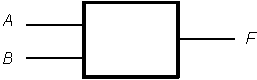
\includegraphics[width=\textwidth]{generic_gate}
  \end{column}
  \begin{column}{.58\textwidth}
    \begin{itemize}\small\itemsep3pt
      \item A gate has one or more inputs and one output set by its function.
      \item \alert{Boolean algebra}: variables take values 0 or 1; complement written $\overline{A}$ or $A'$.
      \item A \alert{truth table} lists output for every input combination; inputs left, output right.
      \item A canonical truth table for $n$ inputs has $2^n$ rows.
    \end{itemize}
  \end{column}
  \end{columns}
\end{frame}

\gateframe{AND Gate}{ANSI_AND}{A\cdot B = AB}
  {0 & 0 & 0 \\ 0 & 1 & 0 \\ 1 & 0 & 0 \\ 1 & 1 & 1 \\}
  {HIGH only when \alert{all} inputs are HIGH. Like switches in \alert{series}: the lamp lights only if both are closed.}

\gateframe{OR Gate}{ANSI_OR}{A + B}
  {0 & 0 & 0 \\ 0 & 1 & 1 \\ 1 & 0 & 1 \\ 1 & 1 & 1 \\}
  {HIGH when \alert{at least one} input is HIGH. Like switches in \alert{parallel}.}

\begin{frame}{NOT Gate (Inverter)}
  \begin{columns}[c]
  \begin{column}{.38\textwidth}
    \centering
    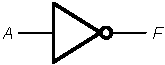
\includegraphics[width=.6\textwidth]{ANSI_NOT}\\[3mm]
    $F = \overline{A}$
  \end{column}
  \begin{column}{.25\textwidth}
    \centering\small
    \begin{tabular}{c|c}
      \toprule
      $A$ & $F$ \\
      \midrule
      0 & 1 \\
      1 & 0 \\
      \bottomrule
    \end{tabular}
  \end{column}
  \begin{column}{.35\textwidth}
    \small One input. Output is the opposite level. The \alert{bubble} at the output denotes inversion.
  \end{column}
  \end{columns}
\end{frame}

\begin{frame}{Switch Models of the Basic Gates}
  \centering
  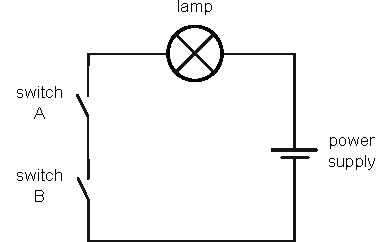
\includegraphics[height=.2\textheight]{switch_AND}\hspace{6mm}
  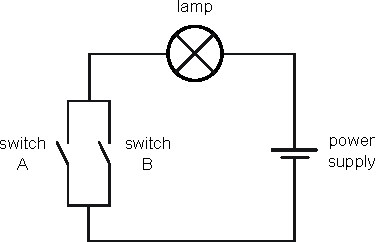
\includegraphics[height=.2\textheight]{switch_OR}\hspace{6mm}
  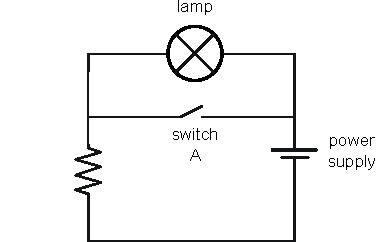
\includegraphics[height=.2\textheight]{switch_NOT}\\[1mm]
  {\small AND: series \hspace{.12\textwidth} OR: parallel \hspace{.1\textwidth} NOT: switch across the lamp}
  \begin{itemize}
    \item Open switch = logic 0; closed switch = logic 1; lamp = output.
    \item This is why digital circuits are called \alert{switching circuits}.
  \end{itemize}
\end{frame}

\begin{frame}{Timing Diagram of a Gate}
  \begin{columns}[c]
  \begin{column}{.55\textwidth}
    \centering
    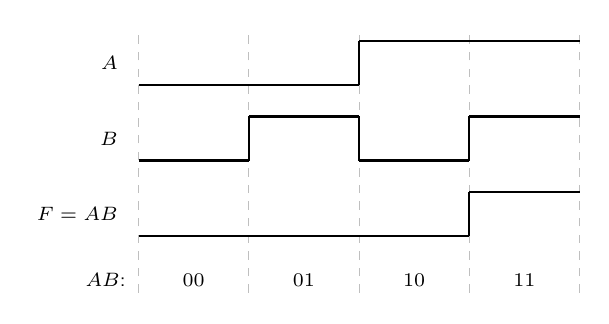
\begin{tikzpicture}[font=\sffamily\scriptsize, x=1.4cm, y=.8cm]
      \foreach \i in {0,...,4} \draw[gray!50, dashed] (\i,-0.3) -- (\i,3.9);
      \wave{3.0}{$A$}{0,0,1,1}
      \wave{1.8}{$B$}{0,1,0,1}
      \wave{0.6}{$F=AB$}{0,0,0,1}
      \foreach \t/\l in {0.5/00,1.5/01,2.5/10,3.5/11} \node at (\t,-0.1) {$\l$};
      \node at (-0.3,-0.1) {$AB$:};
    \end{tikzpicture}
  \end{column}
  \begin{column}{.43\textwidth}
    \begin{itemize}\small\itemsep3pt
      \item A truth table has no notion of time. A \alert{timing diagram} plots levels against time.
      \item Each interval matches one truth-table row.
      \item Inputs on top, outputs below.
    \end{itemize}
  \end{column}
  \end{columns}
\end{frame}

\begin{frame}{Networks of Gates}
  \begin{columns}[c]
  \begin{column}{.42\textwidth}
    \centering
    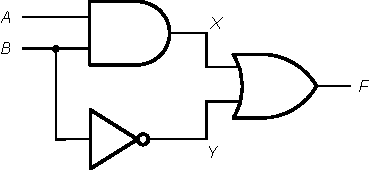
\includegraphics[width=\textwidth]{simplest_net}\\[2mm]
    {\small $X = AB,\quad Y = \overline{B},\quad F = X + Y$}
  \end{column}
  \begin{column}{.56\textwidth}
    \centering
    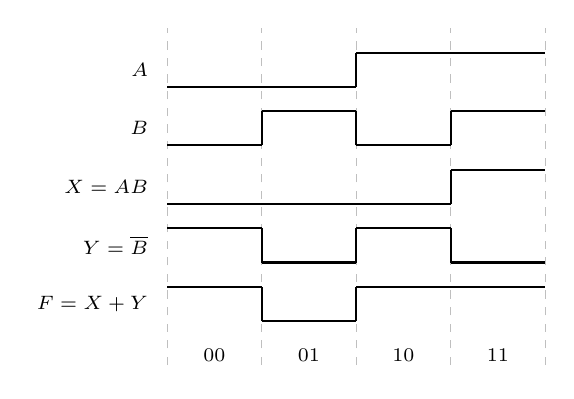
\begin{tikzpicture}[font=\sffamily\scriptsize, x=1.2cm, y=.62cm]
      \foreach \i in {0,...,4} \draw[gray!50, dashed] (\i,-0.3) -- (\i,6.6);
      \wave{5.4}{$A$}{0,0,1,1}
      \wave{4.2}{$B$}{0,1,0,1}
      \wave{3.0}{$X=AB$}{0,0,0,1}
      \wave{1.8}{$Y=\overline{B}$}{1,0,1,0}
      \wave{0.6}{$F=X+Y$}{1,0,1,1}
      \foreach \t/\l in {0.5/00,1.5/01,2.5/10,3.5/11} \node at (\t,-0.1) {$\l$};
    \end{tikzpicture}
  \end{column}
  \end{columns}
  \vspace{1mm}
  {\small $F$ is LOW only when $X$ and $Y$ are both LOW: $A=0,\ B=1$. For $AB = 10$: $X = 0$, $Y = 1$, so $F = 1$.}
\end{frame}

\begin{frame}{More Than Two Inputs}
  \begin{columns}[c]
  \begin{column}{.35\textwidth}
    \centering
    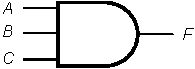
\includegraphics[width=.8\textwidth]{ANSI_AND3}
  \end{column}
  \begin{column}{.62\textwidth}
    \begin{itemize}\small\itemsep3pt
      \item NOT has exactly one input; AND and OR can have many.
      \item AND is 1 only if \alert{every} input is 1; OR is 1 if \alert{any} input is 1.
      \item A 3-input gate has $2^3 = 8$ truth-table rows (000 to 111). The 3-input AND is 1 only on row 111.
    \end{itemize}
  \end{column}
  \end{columns}
\end{frame}

%===============================================================================
\section{Derived Logic Gates}
%===============================================================================

\gateframe{NAND Gate}{ANSI_NAND}{\overline{AB}}
  {0 & 0 & 1 \\ 0 & 1 & 1 \\ 1 & 0 & 1 \\ 1 & 1 & 0 \\}
  {NOT-AND: LOW only when \alert{all} inputs are HIGH. Equivalent to an AND followed by a NOT.}

\gateframe{NOR Gate}{ANSI_NOR}{\overline{A+B}}
  {0 & 0 & 1 \\ 0 & 1 & 0 \\ 1 & 0 & 0 \\ 1 & 1 & 0 \\}
  {NOT-OR: HIGH only when \alert{all} inputs are LOW. Equivalent to an OR followed by a NOT.}

\begin{frame}{NAND Is Universal}
  \begin{columns}[t]
  \begin{column}{.5\textwidth}
    \begin{block}{NOT from NAND}
      \small Tie both inputs together:\\
      $\overline{A \cdot A} = \overline{A}$
    \end{block}
    \begin{block}{AND from NAND}
      \small NAND followed by a NAND wired as NOT:\\
      $\overline{\overline{AB}} = AB$
    \end{block}
  \end{column}
  \begin{column}{.48\textwidth}
    \begin{alertblock}{Universal gates}
      \small Any Boolean function can be built from NAND gates alone, or from NOR gates alone.
    \end{alertblock}
    \vspace{2mm}
    \small Back to the opening question: pick \alert{NAND} (or NOR). One gate type, one part number, every circuit.
  \end{column}
  \end{columns}
\end{frame}

\begin{frame}{Equivalent Forms of NAND and NOR}
  \centering
  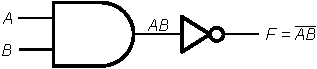
\includegraphics[height=.25\textheight]{equiv_NAND}\hspace{8mm}
  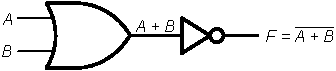
\includegraphics[height=.25\textheight]{equiv_NOR}\\[3mm]
  {\small NAND = AND + NOT \hspace{.15\textwidth} NOR = OR + NOT}
\end{frame}

\gateframe{XOR Gate}{ANSI_XOR}{\overline{A}B + A\overline{B} = A \oplus B}
  {0 & 0 & 0 \\ 0 & 1 & 1 \\ 1 & 0 & 1 \\ 1 & 1 & 0 \\}
  {HIGH when the inputs \alert{differ}. Used in adders and in circuits that detect differences between binary values.}

\gateframe{XNOR Gate}{ANSI_XNOR}{AB + \overline{A}\,\overline{B} = A \odot B}
  {0 & 0 & 1 \\ 0 & 1 & 0 \\ 1 & 0 & 0 \\ 1 & 1 & 1 \\}
  {HIGH when the inputs are \alert{equal}. Opposite of XOR. Useful for comparing bits: output is 1 when they match.}

\begin{frame}{XOR and XNOR from Basic Gates}
  \centering
  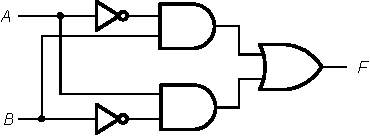
\includegraphics[height=.25\textheight]{equiv_XOR}\hspace{8mm}
  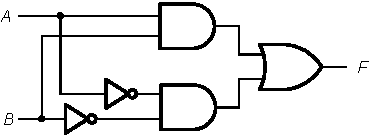
\includegraphics[height=.25\textheight]{equiv_XNOR}\\[3mm]
  {\small XOR from AND, OR, NOT \hspace{.15\textwidth} XNOR = XOR followed by NOT}
\end{frame}

\begin{frame}{Buffers}
  \begin{columns}[c]
  \begin{column}{.3\textwidth}
    \centering
    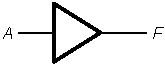
\includegraphics[width=.8\textwidth]{ANSI_BUFFER}
  \end{column}
  \begin{column}{.68\textwidth}
    \begin{itemize}\small\itemsep3pt
      \item One input, one output; $F = A$. The logic value is unchanged.
      \item It supplies more \alert{current} than the source, e.g.\ to drive an LED array, and \alert{isolates} stages.
      \item Larger loads such as relays and solenoids need a proper driver circuit.
    \end{itemize}
  \end{column}
  \end{columns}
  \vspace{1mm}
  \centering
  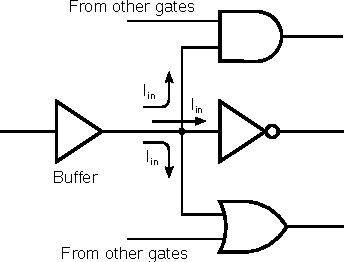
\includegraphics[height=.28\textheight]{buffercurrent}
\end{frame}

\begin{frame}{Tri-State Buffer}
  \begin{columns}[c]
  \begin{column}{.3\textwidth}
    \centering
    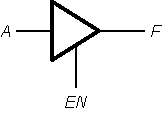
\includegraphics[width=.9\textwidth]{ANSI_TRISTATE_BUFFER}\\[3mm]
    \small\begin{tabular}{cc|c}
      \toprule
      $EN$ & $A$ & $F$ \\
      \midrule
      1 & 0 & 0 \\
      1 & 1 & 1 \\
      0 & X & Hi-Z \\
      \bottomrule
    \end{tabular}
  \end{column}
  \begin{column}{.68\textwidth}
    \begin{itemize}\small\itemsep3pt
      \item An \alert{enable} input controls the output.
      \item Enabled: output follows input. Disabled: \alert{high impedance} (Hi-Z), electrically disconnected.
      \item Several devices can share one line (a bus) if \alert{only one drives it at a time}.
      \item Variants: inverting, and active-low enable $\overline{EN}$.
    \end{itemize}
    \centering
    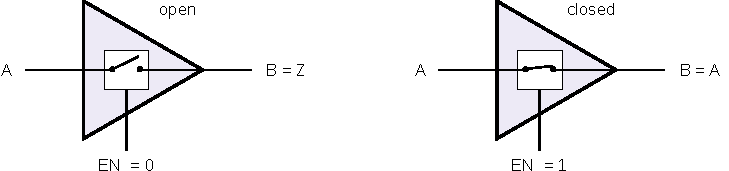
\includegraphics[height=.2\textheight]{tristateequiv}
  \end{column}
  \end{columns}
\end{frame}

\begin{frame}{Buffer Variations}
  \centering
  \begin{columns}[t]
  \begin{column}{.32\textwidth}\centering
    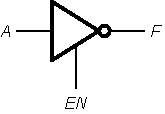
\includegraphics[width=.9\textwidth]{ANSI_INV_TRISTATE_BUFFER}\\[1mm]
    {\scriptsize Inverting, active-high $EN$}\\[1mm]
    \scriptsize\begin{tabular}{cc|c}\toprule $EN$ & $A$ & $F$ \\ \midrule 1 & 0 & 1 \\ 1 & 1 & 0 \\ 0 & X & Hi-Z \\ \bottomrule\end{tabular}
  \end{column}
  \begin{column}{.32\textwidth}\centering
    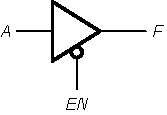
\includegraphics[width=.9\textwidth]{ANSI_TRISTATE_BUFFER_INV_EN}\\[1mm]
    {\scriptsize Non-inverting, active-low $\overline{EN}$}\\[1mm]
    \scriptsize\begin{tabular}{cc|c}\toprule $\overline{EN}$ & $A$ & $F$ \\ \midrule 0 & 0 & 0 \\ 0 & 1 & 1 \\ 1 & X & Hi-Z \\ \bottomrule\end{tabular}
  \end{column}
  \begin{column}{.32\textwidth}\centering
    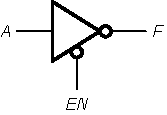
\includegraphics[width=.9\textwidth]{ANSI_INV_TRISTATE_INV_EN}\\[1mm]
    {\scriptsize Inverting, active-low $\overline{EN}$}\\[1mm]
    \scriptsize\begin{tabular}{cc|c}\toprule $\overline{EN}$ & $A$ & $F$ \\ \midrule 0 & 0 & 1 \\ 0 & 1 & 0 \\ 1 & X & Hi-Z \\ \bottomrule\end{tabular}
  \end{column}
  \end{columns}
  \vspace{2mm}
  {\small Each gives signal isolation and controlled drive in a different configuration.}
\end{frame}

%===============================================================================
\section{Boolean Theorems}
%===============================================================================

\begin{frame}{Boolean Algebra and Axioms}
  \begin{itemize}\small\itemsep3pt
    \item George Boole (1854) based it on AND, OR, NOT. Claude Shannon (1930s) applied it to two-state switching circuits.
    \item Theorems simplify expressions, cutting gates, cost and failure points.
  \end{itemize}
  \begin{center}
  \begin{tabular}{cc}
    $0 \cdot 0 = 0$ & $1 + 1 = 1$ \\
    $1 \cdot 1 = 1$ & $0 + 0 = 0$ \\
    $0 \cdot 1 = 1 \cdot 0 = 0$ & $0 + 1 = 1 + 0 = 1$ \\
    $\overline{1} = 0$ & $\overline{0} = 1$ \\
  \end{tabular}
  \end{center}
  {\small Here $+$ is OR, $\cdot$ is AND, and the overbar is NOT.}
\end{frame}

\begin{frame}{Single-Variable Theorems}
  \centering\small\striped
  \begin{tabular}{@{}clcc@{}}
    \toprule
    & \textbf{Theorem} & \textbf{AND form} & \textbf{OR form} \\
    \midrule
    T1 & Annulment & $A \cdot 0 = 0$ & $A + 1 = 1$ \\
    T2 & Identity & $A \cdot 1 = A$ & $A + 0 = A$ \\
    T3 & Idempotency & $A \cdot A = A$ & $A + A = A$ \\
    T4 & Complements & $A \cdot \overline{A} = 0$ & $A + \overline{A} = 1$ \\
    T5 & Involution & \multicolumn{2}{c}{$\overline{\overline{A}} = A$} \\
    \bottomrule
  \end{tabular}
  \begin{itemize}\small\itemsep2pt
    \item \alert{Duality}: swap AND with OR, and 0 with 1, to get the dual theorem.
  \end{itemize}
  \begin{block}{Example: $F = A\cdot A\cdot\overline{A} + 1$}
    \small T3: $A \cdot A = A$. T4: $A\cdot\overline{A} = 0$. So $F = 0 + 1 = 1$. (Directly by T1: anything $+\,1 = 1$.)
  \end{block}
\end{frame}

\begin{frame}{Theorems as Circuits: T1--T3}
  \begin{columns}[c]
  \begin{column}{.32\textwidth}\centering
    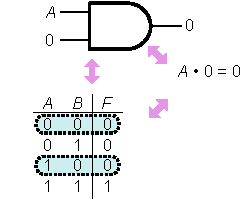
\includegraphics[height=.26\textheight]{boolean-annulment-and}\\{\scriptsize $A\cdot 0 = 0$}\\[2mm]
    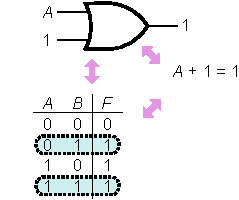
\includegraphics[height=.26\textheight]{boolean-annulment-or}\\{\scriptsize $A + 1 = 1$}
  \end{column}
  \begin{column}{.32\textwidth}\centering
    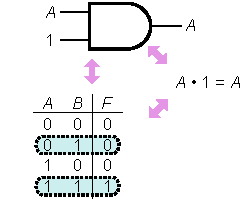
\includegraphics[height=.26\textheight]{boolean-identity-and}\\{\scriptsize $A\cdot 1 = A$}\\[2mm]
    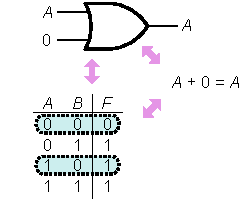
\includegraphics[height=.26\textheight]{boolean-identity-or}\\{\scriptsize $A + 0 = A$}
  \end{column}
  \begin{column}{.32\textwidth}\centering
    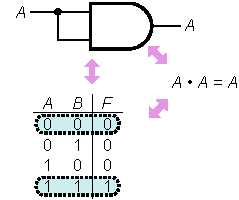
\includegraphics[height=.26\textheight]{boolean-idempotency-and}\\{\scriptsize $A\cdot A = A$}\\[2mm]
    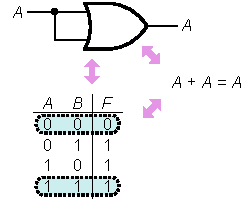
\includegraphics[height=.26\textheight]{boolean-idempotency-or}\\{\scriptsize $A + A = A$}
  \end{column}
  \end{columns}
\end{frame}

\begin{frame}{Theorems as Circuits: T4--T5}
  \begin{columns}[c]
  \begin{column}{.48\textwidth}\centering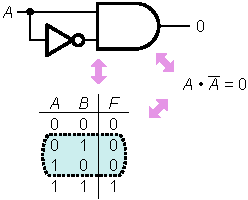
\includegraphics[height=.3\textheight]{boolean-complements-and}\\{\scriptsize $A\cdot\overline{A} = 0$}\end{column}
  \begin{column}{.48\textwidth}\centering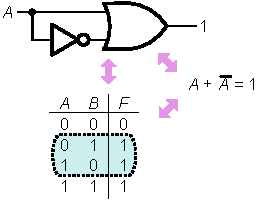
\includegraphics[height=.3\textheight]{boolean-complements-or}\\{\scriptsize $A + \overline{A} = 1$}\end{column}
  \end{columns}
  \vspace{2mm}
  \centering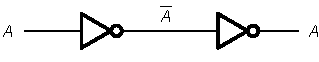
\includegraphics[height=.2\textheight]{boolean-involution}\\{\scriptsize $\overline{\overline{A}} = A$}
\end{frame}

%===============================================================================
\section{Gate ICs}
%===============================================================================

\begin{frame}{Gate Integrated Circuits}
  \begin{columns}[c]
  \begin{column}{.5\textwidth}
    \begin{itemize}\small\itemsep3pt
      \item SSI chips of the \alert{74 series} hold four or six gates each: ``quad'' and ``hex''.
      \item DIP suits labs and breadboards; SOT-23 and DFN fit tight spaces.
      \item DIP14: pins numbered counter-clockwise from pin 1, beside the notch.
      \item Pinouts vary: \alert{always check the datasheet}.
    \end{itemize}
  \end{column}
  \begin{column}{.48\textwidth}
    \centering
    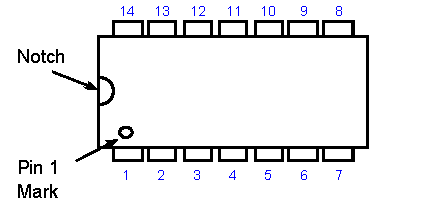
\includegraphics[width=.9\textwidth]{dip-pinout}
  \end{column}
  \end{columns}
\end{frame}

\begin{frame}{74-Series Examples}
  \centering
  \begin{columns}[b]
  \begin{column}{.3\textwidth}\centering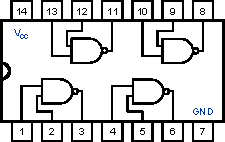
\includegraphics[width=\textwidth]{inside_7400}\\{\scriptsize 74x00 quad NAND}\end{column}
  \begin{column}{.3\textwidth}\centering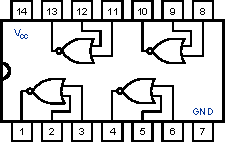
\includegraphics[width=\textwidth]{inside_7402}\\{\scriptsize 74x02 quad NOR}\end{column}
  \begin{column}{.3\textwidth}\centering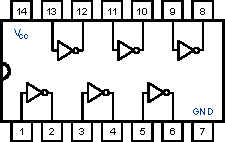
\includegraphics[width=\textwidth]{inside_7404}\\{\scriptsize 74x04 hex inverter}\end{column}
  \end{columns}
  \vspace{4mm}
  \begin{columns}[b]
  \begin{column}{.3\textwidth}\centering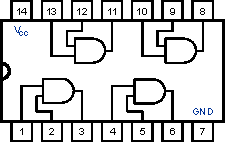
\includegraphics[width=\textwidth]{inside_7408}\\{\scriptsize 74x08 quad AND}\end{column}
  \begin{column}{.3\textwidth}\centering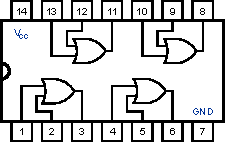
\includegraphics[width=\textwidth]{inside_7432}\\{\scriptsize 74x32 quad OR}\end{column}
  \begin{column}{.3\textwidth}\centering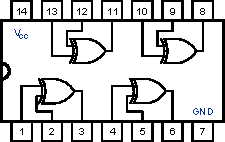
\includegraphics[width=\textwidth]{inside_7486}\\{\scriptsize 74x86 quad XOR}\end{column}
  \end{columns}
\end{frame}

\begin{frame}{Reading a Schematic}
  \begin{columns}[c]
  \begin{column}{.5\textwidth}
    \centering
    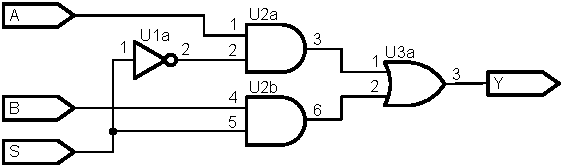
\includegraphics[width=\textwidth]{orcad1}
  \end{column}
  \begin{column}{.48\textwidth}
    \begin{itemize}\small\itemsep3pt
      \item \alert{U1} (74x04): inverter U1a, pins 1--2.
      \item \alert{U2} (74x08): AND gates U2a (pins 1, 2, 3) and U2b (pins 4, 5, 6).
      \item \alert{U3} (74x32): OR gate U3a, pins 1, 2, 3.
      \item The designator names the IC; the letter names the gate inside it.
    \end{itemize}
  \end{column}
  \end{columns}
\end{frame}

%===============================================================================
\section{Measuring Performance}
%===============================================================================

\begin{frame}{Power Consumption}
  \begin{columns}[c]
  \begin{column}{.55\textwidth}
    \begin{block}{CMOS total power = static + dynamic}
      \small
      \[ P_\mathrm{s} = I_\mathrm{dd} V_\mathrm{dd}\quad\text{(leakage)} \]
      \[ P_\mathrm{dyn} = C_L V_\mathrm{dd}^2 f \]
    \end{block}
    \begin{itemize}\small\itemsep2pt
      \item $C_L$: load capacitance; $V_\mathrm{dd}$: supply; $f$: switching frequency.
      \item CMOS idles at very low power; its power rises with $f$.
      \item TTL draws roughly constant power regardless of speed.
    \end{itemize}
  \end{column}
  \begin{column}{.43\textwidth}
    \centering
    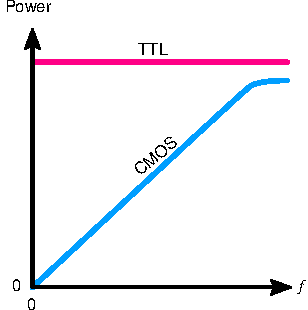
\includegraphics[width=\textwidth]{cmosvsttlpower}
  \end{column}
  \end{columns}
\end{frame}

\begin{frame}{Propagation Delay}
  \begin{columns}[c]
  \begin{column}{.5\textwidth}
    \begin{itemize}\small\itemsep3pt
      \item A gate does not respond instantly. \alert{Propagation delay} is the time from an input transition to the output transition.
      \item $t_\mathrm{PHL}$: output HIGH to LOW. $t_\mathrm{PLH}$: output LOW to HIGH.
    \end{itemize}
    \[ t_\mathrm{pd} = \frac{t_\mathrm{PHL} + t_\mathrm{PLH}}{2} \]
  \end{column}
  \begin{column}{.48\textwidth}
    \centering
    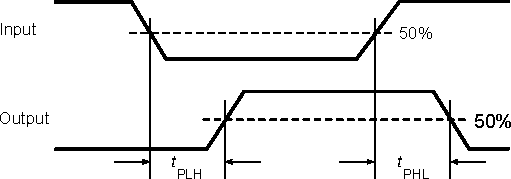
\includegraphics[width=\textwidth]{delay}
  \end{column}
  \end{columns}
  \begin{itemize}\small\itemsep2pt
    \item Typical speed order: inverters, then NAND/NOR, then AND/OR, then XOR/XNOR.
    \item The path with the greatest total delay is the \alert{critical path}; it limits the maximum operating speed.
  \end{itemize}
\end{frame}

%===============================================================================
\section{Alternative Symbols}
%===============================================================================

\begin{frame}{Conventional and Rectangular Symbols}
  \centering
  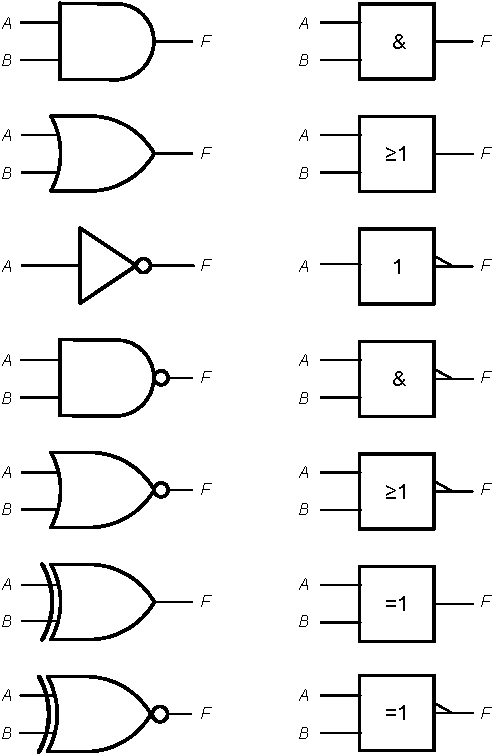
\includegraphics[height=.62\textheight]{all_logic_symbols}
  \begin{itemize}\small
    \item ANSI/IEEE Std 91-1984 rectangular symbols: \texttt{\&} = AND, \texttt{1} = OR, \texttt{=1} = XOR for two inputs. A triangle replaces the bubble.
  \end{itemize}
\end{frame}

%===============================================================================
\section{Summary}
%===============================================================================

\begin{frame}{Summary}
  \begin{itemize}\itemsep3pt\small
    \item A truth table defines a gate's function; the symbol is its graphical form.
    \item \alert{NAND and NOR are universal}: any Boolean function from one gate type.
    \item \alert{Propagation delay} limits speed; the critical path sets the maximum frequency.
    \item Dynamic CMOS power $\approx C V_\mathrm{DD}^2 f$ for constant switching activity.
    \item A \alert{tri-state buffer} adds a Hi-Z state so outputs can share a bus, one driver at a time.
  \end{itemize}
  \begin{block}{Looking ahead}
    Chapter 5 uses Boolean algebra to simplify the logic that these gates implement.
  \end{block}
\end{frame}

\end{document}
